\documentclass[a4paper, parskip=half]{scrartcl}
%\usepackage{libertine}
\usepackage[english]{babel}
\usepackage[utf8]{inputenc}
\usepackage[T1]{fontenc}
\usepackage{amsmath}
\usepackage{tikz}
\usepackage{amsthm}
\usepackage{amssymb}
\usepackage{xfrac}
\usepackage[hidelinks]{hyperref}
\usepackage[super]{nth}
\usetikzlibrary{matrix,calc,3d}
\usetikzlibrary{arrows}
\usetikzlibrary{positioning}
\usepackage{float}

\usepackage{csquotes} 
\usepackage[backend=bibtex8,style=numeric]{biblatex} 
\addbibresource{thesis.bib}

\title{Proton Dynamics in Cavities}
\author{Dominik Wille}

\newcommand{\person}[1]{%
	\textsc{#1}%
}

\newcommand{\effect}[1]{%
	\textbf{#1}%
}

\newcommand{\myImage}[2]{
	\begin{figure}[H]
	\centering
	\includegraphics[width = 0.9\textwidth]{img/#1}
	\caption{#2}
	\label{pic:#1}
	\end{figure}
}

\newcommand{\diff}{\mathop{}\!\mathrm{d}}

\newcommand{\myFigRef}[1]{\textit{\hyperref[#1]{Figure \ref*{#1}}}}

\newcommand{\myEqRef}[1]{\textit{\hyperref[eq:#1]{Equation \ref*{eq:#1}}}}

\newcommand{\mySecRef}[1]{\textit{\hyperref[#1]{Section \ref*{#1}}}}

\newcommand{\myEqLabel}[1]{\label{eq:#1}}

\newcommand{\myEqAnnex}[1]{\;\;\;\mathrm{(Calculation\;In\;Annex)} \myEqLabel{#1}}

\newcommand{\myCite}[1]{\footnote{\cite{#1} \citeauthor{#1} \citetitle{#1} \citeyear{#1}}}

\newcommand\blfootnote[1]{%
  \begingroup
  \renewcommand\thefootnote{}\footnote{#1}%
  \addtocounter{footnote}{-1}%
  \endgroup
}

\begin{document}
\maketitle

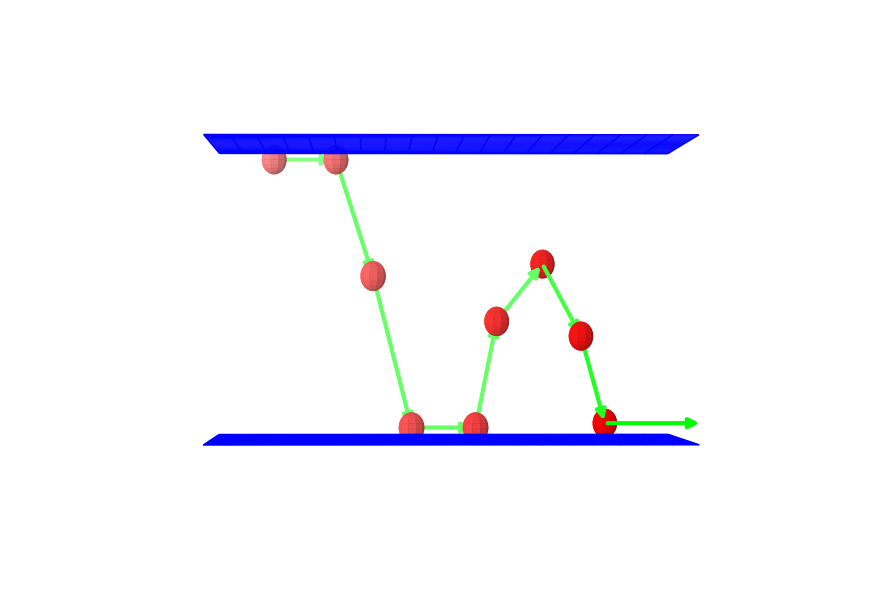
\includegraphics[width=\textwidth]{img/title}

\vfill

\enlargethispage{2cm}
  \parbox[t]{0.45\textwidth}{%
   Freie-Universität-Berlin\\
   Department of Physics\\
   AG Netz
  }
  \parbox[t]{0.55\textwidth}{\raggedleft%
    \nth{1} reviewer: Prof. Dr. Roland R. Netz
  }

\thispagestyle{empty}
\newpage
\tableofcontents
\thispagestyle{empty}
\newpage
% \setcounter{page}{1}

\section{Introduction}%
Recent research on low--frequency ionic currents in nanocavities show fluctuations with $\sfrac{1}{f}$--power spectrums which is also known as pinknoise\myCite{pinknoise}. Smeets et al. made the hypothesis of a link between low-frequency noise and surface charge fluctuations\myCite{paper0}. The assumption in the \effect{absorption-desorption}-model is that charge carriers such as protons can adsorb on surfaces and therefore change the surface's potential. In this thesis, a \effect{Langevin-Simulation} for a proton combined with the absorption-desorption-model is used to demonstrate the probable origin of the widely observed $\sfrac{1}{f}$-fluctuations of ionic--currents.

No interaction between the ion and the two plates such as a coulomb-potential is taken to account. The particle is moreover simulated for the over-damped case. The simulations continue previous analytic calculations by \person{Roland Netz} which obtain correlation functions of the assorbtion-desorbtion-state for infinite cylindrical and infinite planar geometries\myCite{netzpaper}. To determine the correctness of the Langevin-Simulation they are compared to the analytic results for these limiting cases as well as for simple cases such as free particles. Afterwards the simulation is applied to an finite plate geometry which is similar to an nano--pore.

Investigations of the cause of the ionic--current fluctuations could bring hints to extract physical, chemical or even geometrical information concerning the system, they are part of current investigations. Just now some of these fluctuations are the topic of current research\myCite{paper2}. 

The title image shows the visualized position trajectory of a particle on a random walk between two plates in 2-d for different times (The time increases from left to right).


\newpage

\section{Model}
Considered are be $N$ charge carriers such as ions or protons. between to Plates $A$ and $B$. For every particle $i\in\left\lbrace 1,2,...,N \right\rbrace$ the binary function $n_j^i(t)$ stands for the absorption state of the particle on the surface $j$. $n_A^i(t) = 1$ if the particle is adsorbed on Plate $A$ and $n_A^i(t) = 0$ if it is not.

\begin{figure}[H]
\centering
\begin{tikzpicture}[scale=.8, z={(-.707,-.3)}]
    \draw (6,0,0) -- (0,0,0);
    \draw (6,0,0) -- (6,0,-3);
    \draw (6,3,-3) -- (6,3,0);
    \draw (6,3,0) -- (0,3,0);
    \draw (0,3,-3) -- (6,3,-3);
    \draw (0,0,-3) -- (6,0,-3);
    \draw (0,0,0) -- (0,0,-3); 
    \draw (0,3,0) -- (0,3,-3);
    \draw (3,0,-1.5) node{B};
    \draw (3,3,-1.5) node{A};
    \draw[arrows=<->] (0,0.2,0) -- (0,2.8,0);
    \draw (-0.3,1.5,0) node{$H$};
\end{tikzpicture}
\caption{Schematic structure of the system -- The particles which are considered are between these two plates}
\end{figure}
\subsection{Properties}
The number of particles adsorbed on plate $A$ is given by:

\begin{align}
N_A(t) = \sum_{i=1}^N n_A^i(t)
\end{align}

Since experimental investigation measure fluctuations in the potential of nano--structures, especially the auto--correlation function of $N_A(t)$ is of essential importance.

\begin{align}
\langle N_A(0) N_A(t)\rangle &= \sum_{i,j = 1}^N \langle n_A^i(0) n_A^j(t)\rangle\\
&= \sum_{i \neq j}^N \langle n_A^i(0) n_A^j(t)\rangle + \sum_{i =1}^N \langle n_A^i(0) n_A^j(t)\rangle
\end{align}
The particles are usually uncorrelated among each other 
\begin{align}
\langle n_A^i(0) n_A^j(t)\rangle = \langle n_A(0) \rangle\langle n_A(t) \rangle
\end{align}
so let the expectation value of the absorption state for a single particle be:
\begin{align}
\langle n_A^i(t) \rangle &= \langle n_A^i(0) \rangle = p_A \myEqLabel{p_A}\\
\Rightarrow \langle N_A(0) N_A(t)\rangle &= N(N-1)p_a^2 + N\langle n_A(0) n_A(t)\rangle
\end{align}
The only non--trivial quantity to calculate can be defined via the single--ion correlation function $C_{AA}(t)$ which is the probability that a particle is adsorbed at time $t$ given it is adsorbed at time $t=0$.
\begin{align}
C_{AA}(t) &= \langle n_A(0) n_A(t) \rangle / \langle n_A(0) \rangle \\
\Rightarrow \langle N_A(0) N_A(t)\rangle &= N^2p_a^2 + Np_AC_{AA}(t) - Np_a^2
\end{align}
\subsection{Analytic calculations}
The analytic calculations are mostly inherited from \cite{netzpaper} and \cite{netzpaper2}. To understand the used properties in the simulation later on, the key principles should be explained briefly.
\subsubsection{Constructing the single--ion correlation function for a single surface}
For a single surface $A$, one particle that is adsorbed at time $t=0$ can basically keep adsorbed until time $t$ or desorb $n$--times before it is adsorbs again.
\begin{figure}[H]
\centering
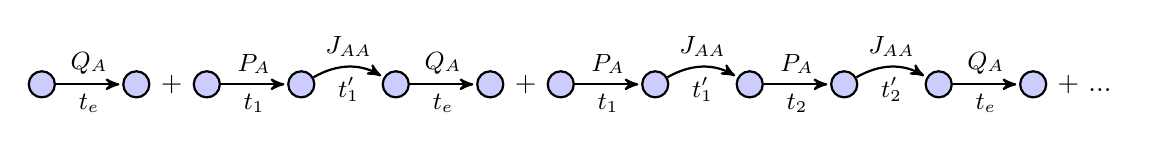
\begin{tikzpicture}[->,>=stealth',shorten >=1pt,auto,node distance=1.2cm,
  thick,main node/.style={circle,fill=blue!20,draw,font=\sffamily\bfseries}]

  \node[main node] (5) {};
  \node[main node] (6) [right of=5] {};
  \node (7) [right=0.0cm of 6] {$+$};

  \path[every node/.style={font=\sffamily\small}]
    (5) edge node [above] {$Q_A$} node [below] {$t_e$} (6);


  \node[main node] (1) [right=0.0cm of 7] {};
  \node[main node] (2) [right of=1] {};
  \node[main node] (3) [right of=2] {};
  \node[main node] (4) [right of=3] {};

  \path[every node/.style={font=\sffamily\small}]
    (1) edge node [above] {$P_A$} node [below] {$t_1$} (2)
    (2) edge[bend left] node[above] {$J_{AA}$} node [below] {$t_1'$} (3)
    (3) edge node [above] {$Q_A$} node [below] {$t_e$} (4);
    
  \node (8) [right=0.0cm of 4] {$+$};
  \node[main node] (9) [right=0.0cm of 8] {};
  \node[main node] (10) [right of=9] {};
  \node[main node] (11) [right of=10] {};
  \node[main node] (12) [right of=11] {};
  \node[main node] (13) [right of=12] {};
  \node[main node] (14) [right of=13] {};
  
  \path[every node/.style={font=\sffamily\small}]
    (9) edge node [above] {$P_A$} node [below] {$t_1$} (10)
    (10) edge[bend left] node[above] {$J_{AA}$} node [below] {$t_1'$} (11)
    (11) edge node [above] {$P_A$} node [below] {$t_2$} (12)
    (12) edge[bend left] node[above] {$J_{AA}$} node [below] {$t_2'$} (13)
    (13) edge node [above] {$Q_A$} node [below] {$t_e$} (14);
    
  \node (15) [right=0.0cm of 14] {$+$ ...};

\end{tikzpicture}
\caption{Illustrated construction of $C_{AA}(t)$ -- Shown are the different trajectories in the state--space which produce the Probability that an particle that is adsorbed at time $t=0$ is adsorbed at time $t$}
\label{fig:ways}
\end{figure}
$J_{AA}(t)$ is the probability for an ion to desorb at time $t=0$ and to return to the surface $A$ at time $t$ for the first time.

$P(t)$ is the distribution that gives probability for an adsorbed ion to desorb at time $t$ for the first time.

$Q_A(t)$ is the survival distribution for an ion to be adsorbed on the surface $A$ over the time span $t=0$ to $t$. Note that this equals the probability that ion desorbes after that time $t$. It is given by:
\begin{align}
Q_A(t) = \int_t^\infty P(t') \diff t'
\end{align}

As illustrated in \myFigRef{fig:ways} $C_{AA}(t)$ is the sum of different paths in the space of states. In other words the probability that a particle is adsorbed at time $t$ given it is adsorbed at time $t=0$ is the sum over the probabilities of all ways on which a particle is adsorbed at time $t=0$ and on time $t$. The probability of one way on the other hand is the product of the probabilities of its parts $Q_A$, $P_A$, and $J_{AA}$.

Generally all that states in $C_{AA}(t)$ of particles could remain for every time smaler than $t$. Therefore it is necessary to vary all these times. 

The expression for $C_{AA}$ \myEqRef{def_Caa}  sums up all variations illustrated in \myFigRef{fig:ways} with general times $t_e$ for $Q(t)$, $t_j$ for $P_A(t)$ and $t_j'$ for $J_{AA}(t)$. In order to obtain the probability at time $t$ the \effect{Dirac-Delta-Function} pics out variants with $\sum_{j} (t_j+t_j') + t_e = t$.

\begin{align}
C_{AA}(t) = &\sum_{i=0}^\infty \Bigg\lbrace \int_0^\infty \diff t_e\, Q_A(t_e) \prod_{j=1}^i \left[ \int_0^\infty \diff t_j\, P_A(t_j) \int_0^\infty \diff t_j'\, J_{AA}(t_j')\right]\notag\\ 
&\delta \left(\sum_{k=1}^i(t_k+t_k') + t_e - t \right) \Bigg\rbrace \myEqLabel{def_Caa}
\end{align}

This expression itself is very though to calculate. But there is common trick to derive the \effect{Laplace-transform} $\widetilde{C}_{AA}(\omega)$ of $C_{AA}(t)$.

\begin{align}
\widetilde{C}_{AA}(\omega) &= \int_0^\infty e^{-\omega t'} \cdot C_{AA}(t') \diff t'
\end{align}

Remember that the integrand in \myEqRef{def_Caa} has only non--zero values for $\sum_{j} (t_j+t_j') + t_e = t$. Therefore it is possible to split the $e^{-\omega t'}$--term.

\begin{align}
e^{-\omega t'} &= e^{-\omega t_e} \cdot \prod_{j=1}^i e^{-\omega t_j} \cdot e^{-\omega t_j'}\\
\Rightarrow  \widetilde{C}_{AA}(\omega) &= \sum_{i=0}^\infty \Bigg\lbrace \int_0^\infty \diff t_e\, e^{-\omega t_e} Q_A(t_e) \prod_{j=1}^i \left[ \int_0^\infty \diff t_j\, e^{-\omega t_j} P_A(t_j) \int_0^\infty \diff t_j'\, e^{-\omega t_j'} J_{AA}(t_j')\right]\notag\\ 
&\delta \left(\sum_{k=1}^i(t_k+t_k') + t_e - t \right) \Bigg\rbrace\\
&= \sum_{i=0}^\infty \Bigg\lbrace \widetilde{Q}_A(\omega) \prod_{j=1}^i \left[\widetilde{P}_A(\omega) \cdot \widetilde{J}_{AA}(\omega) \right]  \Bigg\rbrace \\
&= \sum_{i=0}^\infty \widetilde{Q}_A(\omega) \left[\widetilde{P}_A(\omega) \cdot \widetilde{J}_{AA}(\omega) \right]^i
\end{align}
With the formula for geometric series 
\begin{align}
\sum_{i=0}^{n-1}q^i = \frac{1-q^n}{1-q} 
\end{align}
this becomes the following expression:
\begin{align}
\widetilde{C}_{AA}(\omega) &= \frac{\widetilde{Q}_A(\omega)}{1-\widetilde{P}_A(\omega) \cdot \widetilde{J}_{AA}(\omega)}
\end{align}
\subsubsection{Constructing the single--ion correlation function for two surfaces}
The calculation of $\widetilde{C}_{AA}(\omega)$ for one surface should give a general idea how the laplace-transform of the correlation functions look like.

For instance $\overline{C}_{AA}(\omega)$, $\overline{C}_{BB}(\omega)$, which omit the $\widetilde{Q}_{A/B}(\omega)$ terms, represent trajectories in the state--space where the particle is adsorbed at time $t=0$ and exactly adsorbs at time $t$. 
\begin{align}
\overline{C}_{AA}(\omega) &= \frac{1}{1-\widetilde{P}_A(\omega) \cdot \widetilde{J}_{AA}(\omega)} \\
\overline{C}_{BB}(\omega) &= \frac{1}{1-\widetilde{P}_B(\omega) \cdot \widetilde{J}_{BB}(\omega)} 
\end{align}

States which pass through one time are in the nominator, parts which pass through $n$--times are in the denominator. Parts which are performed equal times can be just multiplied in the laplace-transform.

$\widetilde{C}_{AA}(\omega)$ can be constructed as:

\begin{align}
&\widetilde{C}_{AA}(\omega) = \frac{\overline{C}_{AA}(\omega) \, \widetilde{Q}_{A}(\omega)}{1-\overline{C}_{AA}(\omega)\, \widetilde{P}_A(\omega)\, \widetilde{J}_{AB}(\omega)\, \overline{C}_{BB}(\omega)\, \widetilde{P}_B(\omega)\,\widetilde{J}_{BA}(\omega)}\\
&= \frac{\widetilde{Q}_A(\omega)\left(1 - \widetilde{P}_A(\omega)\, \widetilde{J}_{AA}(\omega) \right)}{\left(1 - \widetilde{P}_A(\omega)\, \widetilde{J}_{AA}(\omega) \right)\left(1 - \widetilde{P}_B(\omega)\, \widetilde{J}_{BB}(\omega) \right) - \widetilde{P}_A(\omega)\, \widetilde{J}_{AB}(\omega)\, \widetilde{P}_B(\omega)\, \widetilde{J}_{BA}(\omega)} \myEqLabel{def_caa}
\end{align}

The new introduced indies stand for the different surfaces, for example $\widetilde{J}_{BA}(\omega)$ is the laplace--transformed of the probability that an ion adsorbed on plate $A$ at time $t=0$ is adsorbs on Plate $B$ at time $t$. 

\person{Roland Netz} show that for infinite plates with surface reaction boundary conditions which in unrescaled units read 
\begin{align}
D \frac{\partial}{\partial x}\widetilde{G}(x, \omega| x_0) \big\vert_{x=x_A} = k_A \widetilde{G}(x, \omega| x_0) \big\vert_{x=x_A} \\
D \frac{\partial}{\partial x}\widetilde{G}(x, \omega| x_0) \big\vert_{x=x_B} = - k_B \widetilde{G}(x, \omega| x_0) \big\vert_{x=x_B} \\
\end{align}
and a $P_A(t)$ which is given by
\begin{align}
P_A(t) &= \frac{1}{\tau_A} e^{-\sfrac{t}{\tau_A}} \myEqLabel{P_t}
\end{align}
the laplace-transform functions read as: 

\begin{align}
\widetilde{P}_A(\omega) &= \frac{1}{1+\tau_A\omega} \\
\widetilde{P}_B(\omega) &= \frac{1}{1+\tau_B\omega} \\
\widetilde{Q}_A(\omega) &= \frac{\tau_A}{1+\tau_A\omega} \\
\widetilde{J}_{AA}(\omega) &= \frac{\widetilde{k}_A \left(1 - \widetilde{k}_B + e^{2\widetilde{H}} (1 + \widetilde{k}_B)\right)}{e^{2\widetilde{H}}(1 + \widetilde{k}_B)(1 + \widetilde{k}_A) - (1 -  \widetilde{k}_B)(1-\widetilde{k}_A)} \\
\widetilde{J}_{AB}(\omega) &= \frac{2e^{\widetilde{H}} \widetilde{k}_A}{e^{2\widetilde{H}}(1 + \widetilde{k}_B)(1 + \widetilde{k}_A) - (1 -  \widetilde{k}_B)(1-\widetilde{k}_A)} \\
\widetilde{J}_{BB}(\omega) &= \frac{\widetilde{k}_B \left(1 - \widetilde{k}_A + e^{2\widetilde{H}} (1 + \widetilde{k}_A)\right)}{e^{2\widetilde{H}}(1 + \widetilde{k}_A)(1 + \widetilde{k}_A) - (1 -  \widetilde{k}_A)(1-\widetilde{k}_B)}
\end{align}

$\widetilde{H} = \sqrt{\sfrac{\omega}{D}} H$ is the rescaled distance of the two plates. The resaceled phenomenological constants $\widetilde{k}_A = k_A / \sqrt{\omega D}$ and $\widetilde{k}_B = k_B / \sqrt{\omega D}$ are the constants of proportionality between the ion boundary flux and the ion boundary density.
\subsubsection{Limiting case}
The limiting case for $k_A = k_B = k \rightarrow \infty$ is of special interest. This case descriptively means that an ion adsorbs in every time if it reaches the boundary condition. To simplify the situation even more, the desorption probability on both surfaces should be the same $\tau_A = \tau_B = \tau$.
\begin{align}
\widetilde{J}_{AA}(\omega) &= \frac{\widetilde{k}^2 \left(e^{2\widetilde{H}} - 1\right) + \widetilde{k}(...)}{\widetilde{k}^2 \left(e^{2\widetilde{H}} - 1\right) + \widetilde{k}(...) + (...)} \rightarrow 1\\
\widetilde{J}_{AB}(\omega) &= \frac{\widetilde{k}(...) + (...)}{\widetilde{k}^2(...) + \widetilde{k}(...) + (...)} \rightarrow 0\\
\end{align}
If the limits of factors exist, the limit of products is the product of the limits. Therefore the limits of $\widetilde{J}_{AA}(\omega)/\widetilde{J}_{AB}(\omega)$ can be used in \myEqRef{def_caa}:
\begin{align}
\Rightarrow \lim_{k\rightarrow\infty} \widetilde{C}_{AA}(\omega) &= \frac{\widetilde{Q}_A(\omega)\left(1 - \widetilde{P}_A(\omega)\, \widetilde{J}_{AA}(\omega) \right)}{\left(1 - \widetilde{P}_A(\omega)\, \widetilde{J}_{AA}(\omega) \right)\left(1 - \widetilde{P}_B(\omega)\, \widetilde{J}_{BB}(\omega) \right) - 0(...)}\\
&= \frac{\widetilde{Q}_A(\omega)}{\left(1 - \widetilde{P}_B(\omega)\, \widetilde{J}_{BB}(\omega) \right)}\\
&= \frac{\frac{\tau}{1+\tau\omega}}{1-\frac{1}{1+\tau\omega}} = \frac{\tau}{1+\tau\omega - 1}\\
&= \frac{1}{\omega} \myEqLabel{analytic_caa}
\end{align}
\newpage
\subsection{Simulation Methods}
The motion of a particle such as a proton in a fluid is primarily  caused by collisions with other particles. This motion firstly was described by \person{Robert Brown} who observed the motion of minute particles of pollen in water and is widely known as \effect{brownian motion}. Simulations for these situations are known as \effect{Brownian-Dynamics-Simulations}.
\subsubsection{Langevin Equation}
The principle of a Brownian-Dynamics-Simulation generally is to consider collisions with other particles as a random forces. And propergate the position of a particle over small time steps $\delta t$.\myCite{book}

Although ions and especially protons, which should be described in the simulation, are not necessarily smaller than the fluid molecules which is the reason why the diffusion constant does not fulfill \person{Einsteins} formula\myCite{brownian}, the general assumption that the motion is caused by random strokes is fulfilled for smaller particles as well. In this document a \effect{Langevin-Simulation} of a particle is used to determine correlations of the adsorption--desorption processes, which can be indirectly measured as conductivity and potential.
 
An approach to describe situations with brownian motion was suggested by \person{Paul Langevin} who added the random force $\mathbf{Z}(t)$ in newtons equation of motion. This stochastic term represents the collision driven force. His equation, the Langevin equation reads:

\begin{align}
m \ddot{\mathbf{r}} = -\lambda\dot{\mathbf{r}} + \mathbf{Z}(t)
\end{align}

where $m$ is the mass of the particle, $\mathbf{r}$ the position of the particle and $\lambda$ the friction constant.

Brownian dynamics can be represented with the so called \effect{overdamped langevin equation} where the $m \ddot{\mathbf{r}}$ term is neglected. The equation for the prevailing situation therefore is:

\begin{align}
\lambda\dot{\mathbf{r}} = \mathbf{Z}(t)
\end{align}

In order to get an iterable expression this expression is discretizised in time intervals $\Delta t$:

\begin{align}
\int_t^{t+ \delta t} \dot{\mathbf{r}}(t')\, dt' &= \int_t^{t+ \Delta t} \frac{\mathbf{Z}(t')}{\lambda}\, dt' \\
\mathbf{r}(t + \delta t) - \mathbf{r}(t) &= \frac{1}{\lambda} \int_t^{t+ \Delta t} \mathbf{Z}(t)\, dt'\\
\mathbf{r}(t + \delta t) - \mathbf{r}(t) &\cong \boldsymbol{\zeta}(t, \varepsilon)
\end{align}

In the discussed 1--dimensional case $\varepsilon$ is the mean step size and $\boldsymbol{\zeta}(t, \varepsilon)$ is one random vector. For a simple random walk with fixed step size this will be $\varepsilon$ or $-\varepsilon$ with a chance of $50\%$ each. For a gaussian random walk this will be some value $s$ with a probability:

\begin{align}
P(s) = \frac{1}{\varepsilon \sqrt{2\pi}} e^{-\sfrac{s^2}{2\varepsilon^2}}
\end{align} 

The position of a particle at time $t + \Delta t$ can easily derived from its position at time $t$.

\begin{align}
\mathbf{r}(t + \delta t) = \mathbf{r}(t) + \boldsymbol{\zeta}(t, \varepsilon)
\end{align}

\subsubsection{Connection to diffusion}
The probability density function for both mentioned types of \effect{random walks} fulfill the diffusion equation (\textit{Note: }$n = \sfrac{t}{\delta t}$):
\begin{align}
\frac{\partial}{\partial t} \rho(x,t) &= D \frac{\partial^2}{\partial x^2 } \rho(x,t) \myEqAnnex{diffusion_PDE} \\
\mathrm{with} \, \, \,\, D &= \frac{\varepsilon^2}{2 \delta t} \myEqLabel{def:D}
\end{align}
What means that a random walk can also be seen as a diffusion process. The exact form of the probability density functions is discussed below.
\subsubsection{Fixed step size}
The motion which is performed in the langevin simulation is widely known as a \effect{random walk}. The simplest variant is as mentioned before to choose $\varepsilon$ or $-\varepsilon$ with a chance of $50\%$ each. The probability $p(x, n)$ that a random walk with discrete steps of length $\varepsilon$ comes to a position $x$ after $n$ steps. Is given by:

\begin{align}
p(x, n) = \frac{\mathrm{Number\, of\, ways\, to\, position\,} x}{\mathrm{Total\, number\, of\, ways}} = \frac{N_x}{N}
\end{align}

Since there are 2 possible successors for every position the total number of ways  doubles every step.

\begin{align}
N = 2^n
\end{align}

The number of ways to the position $x$ after n steps can be obtained by \effect{Pascal's triangle}.

\begin{figure}[H]
\centering
\begin{tikzpicture}[description/.style={fill=white,inner sep=2pt}]
\matrix (m) [matrix of math nodes, row sep=1.5em,
column sep=0.3em, text height=1.5ex, text depth=0.25ex,
nodes={
        minimum width=1.0cm
    },
]
{%
\mathrm{Step/Position} &-3\varepsilon &-2\varepsilon & -1\varepsilon & 0 & \varepsilon & 2\varepsilon &3\varepsilon \\
0 & & & & 1 & & & \\
1 & & & 1 & & 1 & & \\
2 & & 1 & & 2 & & 1 &\\
3 & 1 & & 3 & & 3 & & 1\\};
\path[-] (m-2-5) edge (m-3-4)
		 (m-2-5) edge (m-3-6)
		 (m-3-4) edge (m-4-5)
		 (m-3-4) edge (m-4-3)
		 (m-3-6) edge (m-4-7)
		 (m-3-6) edge (m-4-5)
		 (m-5-6) edge (m-4-5)
		 (m-5-4) edge (m-4-3)
		 (m-5-8) edge (m-4-7)
		 (m-5-6) edge (m-4-5)
		 (m-5-6) edge (m-4-5)
		 (m-5-2) edge (m-4-3)
		 (m-5-6) edge (m-4-7)
		 (m-5-4) edge (m-4-5);
\end{tikzpicture}
\caption{Pascal's triangle -- The numbers stand for the number of ways to its position. the distance from the initial position of every point is scaled on top.}
\end{figure}

\begin{align}
N_x &= \binom{n}{k}\\
\mathrm{with} \, \, \,\, k &= \frac{1}{2}\left(\frac{x}{\varepsilon} + n \right)
\end{align}

Therefore $p(x,n)$ follows as:

\begin{align}
p(x,n) = \binom{n}{k} \cdot 2^{-n}
\end{align}
A consequence of the \effect{de Moivre–Laplace theorem} is that for large numbers of steps $(n\rightarrow\infty)$ this expression can be approximated with the following gaussian curve:

\begin{align}
p(x,n) \cong \sqrt{\frac{2}{n \pi}} e^{-\sfrac{x^2}{2\varepsilon^2 n}} \myEqAnnex{moivre_laplace_theorem}
\end{align}

The probability function $p(x,n)$ has valid values only for values 
\begin{align}
x \in \{x\; |\; x = z \cdot 2 \varepsilon + \varepsilon\, (n\,\mathrm{mod}\, 2),\, z \in \mathbb{Z} \wedge |x| \leq n \varepsilon\} 
\end{align}
For other values $x$ the probability is $0$. This means that there is only one value per $2\epsilon$ interval, therefore the probability density function $\rho(x,n)$ is:
\begin{align}
\rho(x,n) = \frac{1}{2\varepsilon}\; p(x,n) = \frac{1}{\varepsilon\sqrt{2\pi n}} e^{-\sfrac{x^2}{2\varepsilon^2 n}} \myEqLabel{rho_binom}
\end{align}
Which is the normal distribution with $\mu = 0;\;\; \sigma =  \varepsilon\sqrt{n}$.

\subsubsection{Gaussian random walk}
The probability density function for a gaussian random walk with mean step size $\varepsilon$ has exactly the same form as the for fixed step size $\varepsilon$.
\begin{align}
\rho(x,n) = \frac{1}{\varepsilon\sqrt{2\pi n}} e^{-\sfrac{x^2}{2\varepsilon^2 n}} \myEqLabel{rho_gauss}
\end{align}
This can easily be shown with a mathematical induction for $p(x,n)$. Note that because every position is possible the probability 
\begin{align}
p(x,n) = 0 
\end{align}
because that means that the number of possible positions is infinite.

\textbf{Base case} ($n = 1$)\textbf{:}
\begin{align}
\rho(x,1) = \frac{1}{\varepsilon\sqrt{2\pi}} e^{-\sfrac{x^2}{2\varepsilon^2}}
\end{align}
Which is exactly the expression of a gaussian distributed 1--dimensional random vector with $\varepsilon$ variance. $\checkmark$

\textbf{Inductive step} ($n + 1$)\textbf{:}
\begin{align}
\rho(x,n+1) &= \int_{-\infty}^\infty \frac{1}{\varepsilon\sqrt{2n\pi}}\, e^{-\sfrac{x'^2}{2n\varepsilon^2}} \cdot \frac{1}{\varepsilon\sqrt{2\pi}}\, e^{-\sfrac{(x - x')^2}{2\varepsilon^2}} \diff x'\\
&= \frac{1}{\varepsilon\sqrt{2(n+1)\pi}}\, e^{-\sfrac{x^2}{2(n+1)\varepsilon^2}} \myEqAnnex{gauss_random_walk}
\end{align}

\subsubsection{Simple random walk vs. Gaussian random walk}

For all relevant simulations a gaussian random walk was used. Even if the distribution density in \myEqRef{rho_binom} and \myEqRef{rho_gauss} becomes equivalent for large numbers of steps the gauss distribution represents a much more natural motion of the particle. Moreover much smaller step sizes what means more steps in the simulation are necessary to allow small motions of the particle. And since performance of the simulation is not an issue the gaussian random walk is just superior the simple random walk. Below figures show example random walks between two plates at $x = \pm 1$.

\myImage{fixed_pos}{Position of a particle performing a simple random walk -- The fixed step size causes a discretizised position of the particle}

\myImage{gauss_pos}{Position of a particle perfoming a gaussian random walk -- The position of the particle is not discretizised as like in the nature}

and since the calculated $\rho(x,n+1)$ is the same as $\rho(x,n)$ in \myEqRef{rho_gauss} the expression is proofed. $\checkmark$
\subsubsection{Mean square distance}
The expectation value for $x$ after $n$ steps $\langle x_n\rangle = 0$. What can be derived from:
\begin{align}
\langle x_n\rangle = \int_{-\infty}^\infty x \cdot \rho(x,t)\diff x = 0
\end{align}
But the \effect{Mean Square Distance} $\langle x_n^2\rangle$ (MSD) fulfills the following expression:
\begin{align}
\langle x_n^2\rangle = \int_{-\infty}^\infty x^2 \cdot \rho(x,t)\diff x = 2 D t \myEqAnnex{MSD}
\end{align}

\newpage
\section{Investigation}
\subsection{Tests of the simulation}
\subsubsection{MSD}
A very simple test is to check if the simulation of a particle without any barriers has a linear growing MSD as a function of performed steps. \myFigRef{pic:mean_square} shows the average squared distance $x_n^2$ for different numbers of runs compared to the analytic expression \myEqRef{MSD_n}. The parameters were:
\begin{center}
\begin{tabular}{c|c}
Parameter & Value \\\hline
$D$ & 0.1 \\
$\delta t$ & 20 \\
$x(n=0)$ & 0 \\
$n_{\mathrm{max}}$ & 400
\end{tabular}
\end{center}
Note that $\varepsilon$ is determined by \myEqRef{def:D}.

The expectation is that for large numbers of runs the mean square converges against the following analytic expression derived from \myEqRef{MSD}:
\begin{align}
\langle x_n^2\rangle (t) &= 2 D t \\
\Rightarrow\langle x_n^2\rangle (n) &= 2 D \delta t \cdot n \myEqLabel{MSD_n}
\end{align}
\myImage{mean_square}{MSD over time -- The more values are taken into account to calculate the MSD the closer it gets to the analytic expression in \myEqRef{MSD_n}}

\newpage
\subsubsection{Infinite plates}
The system which is simulated consists of two infinite plates A and B with distance $H$. Between the two plates there is fluid which surrounds the simulated ion. In the model the ion adsorbs at the surface of the two plates with the probability $p$ and desorbs with an exponential decaying probability $P(t)$ given by:
\begin{align}
P(t) = \frac{1}{\tau}e^{- \sfrac{t}{\tau}} \myEqLabel{adsorb_dist}
\end{align}

The probability density for two infinite plates where the particle can adsorb looks for $t\rightarrow \infty$ is shown in the figure below. The plates are again at $x = \pm 1$.
\myImage{probability_density}{Probability density for two plates located at $x = \pm 1$ -- The implementation of the boundary causes a reduced density near the plates}
The expectation for a reflecting plate would be a constant probability density function. The given probability in \myFigRef{pic:probability_density} density function has some important differences which maybe dues to the implementation of the surface reaction boundary condition. 

It was implemented that the particle adsorbs when it crosses one plate with the probability $p$ which was chosen as $0.3$ here. 
If the particle adsorbs it keeps adsorbed for an exponential distributed time as \myEqRef{adsorb_dist}. After the time the particle keeps adsorbed the langevin simulation continues from that position on the plate. If the first step goes through the plate again the particle adsorbs again in the next step.

This directly implies that there will be high probability that the particle is at the position of a plate, which causes the very high values of $\rho(x)$ at $x = \pm 1$, see in \myFigRef{pic:probability_density}. On the other hand the probability that the particle is close to a plate but not adsorbed is significant smaller than that it is somewhere else between the plates. This maybe dues to the implementation of the boundary condition as well, because all movements that would crosses a plate end up on the position of the plate here. So trajectories that would include a reflection process at the boundaries drop out for adsorbing plates. 


\subsubsection{Correlation functions}
For a geometry with two plates there is a an analytic expression for the Correlation functions $C_{AA}(t)$ and $C_{AB}(t)$ which represent the probability for an ion to be adsorbed at time $t$ on plate $\mathrm{A}/\mathrm{B}$ given that it was adsorbed on plate $\mathrm{A}$ at time $t=0$.

These correlation functions can easily be obtained from the langevin simulation by analyzing the trajectories of the particle. 

Afterwards the values of the correlation function $C_{AA}(t)$ can be calculated as the number of time intervals with length $t$ where the ion is adsorbed on plate $\mathrm{A}$ at the beginning and at the end over the total number of intervals.

Similarly the values of the correlation function $C_{AB}(t)$ can be calculated as the intervals with length $t$ where the ion is adsorbed on plate $\mathrm{A}$ at the beginning and on plate $\mathrm{B}$ at the end over the total number of intervals.

The correlation functions were obtained from a single simulation. For all correlation functions the values of the correlation function $C(t)$ for different times $t$ were calculated as:

\begin{align}
  C_{ij}(t) = \frac{\int_0^{t_{max}-t} S_i(t') \cdot S_j(t' + t) \diff t'}{\int_0^{t_{max}-t} S_i(t') \diff t'}
\end{align}

Where $S_{i/j}(t) = 1$ if the particle has the state at the beginning/end of an interval and $S_{i/j}(t) = 0$ otherwise.

\subsubsection{Parameters of the simulation}
The run for the comparison with the analytic calculations was performed with the following parameters:
\begin{center}
\begin{tabular}{c|c}
Parameter & Value \\\hline
$D$ & 0.1 \\
$\delta t$ & 0.1 \\
$\tau$ & 1.0 \\
$p$ & 1.0 \\
$H$ & 1.0
\end{tabular}
\end{center}

where $D$ the diffusion constant, $\delta t$ the step size, $\tau$ the exponential decay constant for the desorption probability, $p$ the probability that a particle at the boundary adsorbs and $s$ is the plate distance. The initial position for this lagevin--simulation is not relevant for the correlation functions. 

\subsubsection{Interpretation}\label{interpretation}

Also the behavior of the correlation functions in \myFigRef{pic:caa_cab} is easily explainable. Obviously $C_{AA}(t)$ starts from $1$ because by definition it is definitely adsorbed at time $t=0$ on Plate $A$. $C_{AB}(t)$ and $C_{AD}(t)$ start from $0$ because if a particle is adsorbed on plate $A$ it is neither possible that it is adsorbed on plate $B$ nor it is desorbed. For $t \rightarrow \infty$ the adsorbed--desorbtion--state wont depend on the state at time $t = 0$ therefore the correlation functions $C_{AA}(t)$ and $C_{AB}(t)$ become stationary on a finite probability. This probability was called $p_A$ in \myEqRef{p_A}. Also the relation $C_{AD}(t) = 1 - C_{AA}(t) - C_{AB}(t)$ is fulfilled what implies that $C_{AD}(t)$ becomes stationary for $t \rightarrow \infty$ at a finite probability as well. It is $1 - p_A - p_B$.

\subsubsection{Comparison}
In order to compare these correlation functions with its analytic equivalents they need to be Laplace transformed. To obtain easy expressions for the Laplace transformed functions they are fitted with the functions of the following type:

\begin{align}
C(t) &= \sum_{i=0}^{n} c_i \cdot e^{b_i \cdot t} \myEqLabel{fit}
\end{align}

To determine the constants $c_i$ and $b_i$ the \verb+scipy.optimize.curve_fit+ in Phython was used which uses non-linear least squares to fit a function\myCite{curvefit}. For $C_{AA}$ and $C_{AB}$ \myEqRef{fit} was used as a fitting curve with $n=4$ and $n = 4$.

\myImage{caa_cab}{Correlation Functions and its fits -- The behavior of the Correlation functions can be explained very well See \mySecRef{interpretation}}

For the simple exponential expression in \myEqRef{fit} the Laplace transformed can be obtained via:
\begin{align}
F(t) &= c_i \cdot e^{b_i \cdot t} \\
\widetilde{F}(\omega) &= \int_0^\infty c_i \cdot e^{b_i\cdot x} \cdot e^{-\omega\cdot t}\diff t \\
&= \frac{ci}{\omega - b_i}\;\;\;\; \mathrm{(only\; for\,\,\,\, } b_i > \omega \mathrm{)} \myEqLabel{laplace}
\end{align}

The Laplace transform correlation functions follow as:
\begin{align}
\widetilde{C}(\omega) = \sum_{i=0}^n \frac{c_i}{\omega - b_i}
\end{align}

To get an idea of the accuracy of the Laplace transform of the fitted correlation functions also the error of the determined parameters $c_i$ and $b_i$ should considered here.

\begin{align}
\Delta\widetilde{C}(\omega) = \sqrt{\sum_{i=0}^\infty \left(\frac{\Delta c_i}{c_i} \right)^2 + \left( \frac{\Delta b_i}{(\omega - b_i)^2}\right)^2} \cdot \widetilde{C}(\omega)
\end{align}

The comparison between that and the analytic result for $\widetilde{C}_{AA}(\omega)$ is shown on the log--log--plot below. The analytic laplace transform correlation function is given by \myEqRef{analytic_caa}:

\begin{align}
\Delta\widetilde{C}_{AA}(\omega) = \frac{1}{\omega}
\end{align}

\myImage{compare_lac}{Comparsion of the laplace transform correlation function $\widetilde{C}_{AA}(\omega)$ -- The result of the Langevin--Simulation is identical to the analytical result}

The errorbars in the figure above are obtained from the variance of the fitting parameters $c_i$ and $b_i$ which are defined for every time $t$ so there generally has to be an error bar for every time $t$. Those considered here, stand only exemplary for these other errorbars. The positions of the errorbars is chosen to get a nice plot they are not the only data points. 

The figure above makes clear that in the uncertainty of the fitting curve the results are identical. Note that for $\omega \rightarrow b_i$ The fitting function is not properly defined (See \myEqRef{laplace}). That means that the divergence at these values may only be caused by the fitting method.

\newpage
\subsection{Finite plates}

\begin{figure}[H]
\centering
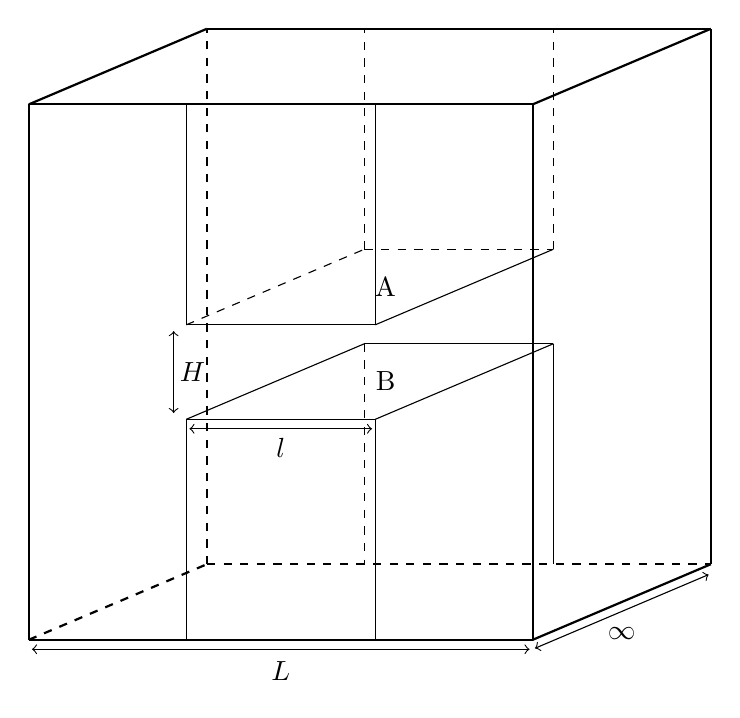
\begin{tikzpicture}[scale=.4, z={(-.707,-.3)}]
    \draw (6,0,2.5) -- (0,0,2.5);
    \draw (6,0,2.5) -- (6,0,-5.5);
    \draw (6,3,-5.5) -- (6,3,2.5);
    \draw (6,3,2.5) -- (0,3,2.5);
    \draw (0,0,-5.5) -- (6,0,-5.5);
    \draw (0,0,2.5) -- (0,0,-5.5); 
    \draw[dashed] (0,3,-5.5) -- (6,3,-5.5);
    \draw[dashed] (0,3,2.5) -- (0,3,-5.5);
    
    \draw (0,3,2.5) -- (0,10,2.5);
    \draw[dashed] (0,3,-5.5) -- (0,10,-5.5);
    \draw[dashed] (6,3,-5.5) -- (6,10,-5.5);
    \draw (6,3,2.5) -- (6,10,2.5);
    \draw (0,0,2.5) -- (0,-7,2.5);
    \draw[dashed] (0,0,-5.5) -- (0,-7,-5.5);
    \draw (6,0,-5.5) -- (6,-7,-5.5);
    \draw (6,0,2.5) -- (6,-7,2.5);
    
    
    \draw[thick] (-5,10,2.5) -- (11,10,2.5);
    \draw[thick] (-5,10,-5.5) -- (11,10,-5.5);
    \draw[thick] (-5,10,2.5) -- (-5,10,-5.5);
    \draw[thick] (11,10,2.5) -- (11,10,-5.5);    
    \draw[thick] (-5,-7,2.5) -- (11,-7,2.5);
    \draw[thick,dashed] (-5,-7,-5.5) -- (11,-7,-5.5);
    \draw[thick,dashed] (-5,-7,2.5) -- (-5,-7,-5.5);
    \draw[thick] (11,-7,2.5) -- (11,-7,-5.5);
    \draw[thick] (-5,-7,2.5) -- (-5,10,2.5);    
    \draw[thick] (11,-7,2.5) -- (11,10,2.5);
    \draw[thick] (11,-7,-5.5) -- (11,10,-5.5);
    \draw[thick,dashed] (-5,-7,-5.5) -- (-5,10,-5.5);
    
    \draw[arrows=<->] (0.1,-0.3,2.5) -- (5.9,-0.3,2.5);
    \draw[] (3,-0.9,2.5) node{$l$};
    \draw[arrows=<->] (-4.9,-7.3,2.5) -- (10.9,-7.3,2.5);
    \draw[] (3,-8.0,2.5) node{$L$};
    \draw[arrows=<->] (11,-7.3,2.4) -- (11,-7.3,-5.4);
    \draw[] (11,-8,-1.5) node{$\infty$};
    
    \draw (3.5,0,-1.5) node{B};
    \draw (3.5,3,-1.5) node{A};
    \draw[arrows=<->] (-0.4,0.2,2.5) -- (-0.4,2.8,2.5);
    \draw (0.2,1.5,2.5) node{$H$};
\end{tikzpicture}
\caption{Schematic structure of the finite plate system}
\end{figure}

\myImage{limited_correlation}{Correlation functions for a finite plate system}

\newpage
\section{Conclusion}



\newpage
\section{Annex}
\myEqRef{diffusion_PDE}
\begin{align}
\rho(x,t) &= \frac{1}{\varepsilon\sqrt{2\pi\sfrac{t}{\delta t}}}\; e^{-\frac{x^2 \delta t}{2 \varepsilon^2 t}} \\
\frac{\partial}{\partial t} \rho(x,t) &= - \frac{1}{2t} \rho(x,t) + \frac{x^2 \delta t}{\varepsilon^2t^2} \rho(x,t) \\
&= \frac{1}{2} \left(\frac{x^2 \delta t}{\varepsilon^2t^2} - \frac{1}{t} \right)\rho(x,t) \\
\frac{\partial^2}{\partial x^2} \rho(x,t) &= \frac{\partial}{\partial x} \left(-\frac{x\delta t}{\varepsilon^2t} \right) \rho(x,t) \\
&= -\frac{\delta t}{\varepsilon^2t} \rho(x,t) + \frac{x^2\delta t^2}{\varepsilon^4 t^2} \rho(x,t) \\
&= \frac{\delta t}{\varepsilon^2}\left(\frac{x^2 \delta t}{\varepsilon^2 t^2} - \frac{1}{t}\right) \rho(x,t) \\
\frac{\partial}{\partial t} \rho(x,t) &= D \frac{\partial^2}{\partial x^2 } \rho(x,t)\\
\Rightarrow \frac{1}{2} &= D \cdot \frac{\delta t}{\varepsilon^2}\\
\Leftrightarrow D &= \frac{\varepsilon^2}{2\delta t}
\end{align}

\myEqRef{moivre_laplace_theorem}
\begin{align}
p(x,n) &= \binom{n}{k} \cdot 2^{-n}\;\;\;\; \mathrm{with}\;\;\; k = \frac{1}{2}\left(n+\frac{x}{\varepsilon}\right)\\
&= \frac{n!}{k!(n-k)!}\cdot 2^{-n}\\
\mathrm{with}\;\;\; n! &\cong \sqrt{2\pi n}\;n^ne^{-n}\tag{Stirling's\;formula}\\
\Rightarrow \;\;\; p(x,n) &\cong \frac{\sqrt{2\pi n}\;n^ne^{-n}}{\sqrt{2\pi k}\;k^ke^{-k} \sqrt{2\pi(n-k)}\;(n-k)^{n-k}e^{k-n}} \cdot 2^{-n}\\
&= \left(\frac{\sqrt{2\pi n}}{\sqrt{2\pi k}\;\sqrt{2\pi(n-k)}} \right) \underbrace{\left(\frac{e^{-n}}{e^{-k}\;e^{k-n}}\right)}_{=1} \left( \frac{n^n}{k^k(n-k)^{n-k}}\right)\cdot 2^{-n}\\
&= \sqrt{\frac{2n}{\pi(n+\sfrac{x}{\varepsilon})(n-\sfrac{x}{\varepsilon})}} \cdot \left(\frac{n}{2} \right)^k \cdot \left(\frac{n}{2} \right)^{n-k} \notag\\
&\;\;\;\;\cdot \left( \frac{1}{2}\left( n+\sfrac{x}{\varepsilon}\right) \right)^{-\frac{1}{2}(n+\sfrac{x}{\varepsilon})} \cdot \left( \frac{1}{2}\left( n-\sfrac{x}{\varepsilon}\right) \right)^{-\frac{1}{2}(n-\sfrac{x}{\varepsilon})} \\
&= \sqrt{\frac{2n}{\pi \left(n^2 - \left( \sfrac{x}{\varepsilon} \right)^2 \right)}} \cdot \left( \frac{n}{n+\sfrac{x}{\varepsilon}}\right)^{-\frac{1}{2}(n+\sfrac{x}{\varepsilon})} \cdot \left( \frac{n}{n-\sfrac{x}{\varepsilon}}\right)^{-\frac{1}{2}(n-\sfrac{x}{\varepsilon})} \\
&= \sqrt{\frac{2n}{\pi \left(n^2 - \left( \sfrac{x}{\varepsilon} \right)^2 \right)}} \cdot \left( 1 + \frac{x}{\varepsilon n}\right)^{-\frac{1}{2}(n+\sfrac{x}{\varepsilon})} \cdot \left( 1 - \frac{x}{\varepsilon n}\right)^{-\frac{1}{2}(n-\sfrac{x}{\varepsilon})} \\
\mathrm{use} \;\;\; x &= e^{\ln(x)}\\
\Rightarrow \;\;\; p(x,n) &\cong \sqrt{\frac{2}{\pi n\left(1 - \left( \frac{\sfrac{x}{\varepsilon}}{n} \right)^2 \right)}} \notag\\
&\;\;\;\;\cdot \exp\!\left\lbrace -\frac{n}{2}\left( 1+\frac{\sfrac{x}{\varepsilon}}{n} \right) \, \ln\!\left(1 + \frac{\sfrac{x}{\varepsilon}}{n} \right) -\frac{1}{2}(n-\sfrac{x}{\varepsilon})\, \ln\!\left(1 - \frac{\sfrac{x}{\varepsilon}}{n} \right) \right\rbrace \\
\mathrm{for}\;\;\; n &\rightarrow\infty \; \Rightarrow \; \alpha \rightarrow 0 \;\;\; \alpha := \frac{\sfrac{x}{\varepsilon}}{n}\; \\ 
&\Rightarrow\;\;  1-\alpha^2 \rightarrow 1 + ... \; \\
&\mathrm{and}\;\,\ln\!\left(1+\alpha\right) \rightarrow \alpha - \frac{1}{2}\alpha^2 + ... \\
\Rightarrow \;\;\; p(x,n) &\cong \sqrt{\frac{2}{n\pi}} \cdot \exp\!\left\lbrace-\frac{n}{2}\left[\left(1+\alpha\right)\left(\alpha - \frac{1}{2} \alpha^2 \right) +\left(1-\alpha\right)\left(-\alpha - \frac{1}{2} \alpha^2 \right)\right] \right\rbrace\\
&= \sqrt{\frac{2}{n\pi}} \cdot \exp\!\left\lbrace-\frac{n}{2}\left[\alpha -\frac{1}{2} \alpha^2 + \alpha^2 - \alpha - \frac{1}{2} \alpha^2 + \alpha^2 + \mathcal{O}(\alpha^3)\right] \right\rbrace \\
&\cong \sqrt{\frac{2}{n\pi}} \cdot \exp\!\left\lbrace-\frac{n}{2}\left[\alpha^2\right] \right\rbrace\\
&= \sqrt{\frac{2}{n\pi}} \cdot e^{-\sfrac{x^2}{2\varepsilon^2n}} 
\end{align}

\myEqRef{gauss_random_walk}
\begin{align}
p(x,n+1) &= \int_{-\infty}^\infty \frac{1}{\varepsilon\sqrt{2n\pi}}\, e^{-\sfrac{x'^2}{2n\varepsilon^2}} \cdot \frac{1}{\varepsilon\sqrt{2\pi}}\, e^{-\sfrac{(x - x')^2}{2\varepsilon^2}} \diff x'\\
&= \frac{1}{\varepsilon^2\sqrt{4\pi^2n}} \, \int_{-\infty}^\infty e^{-\frac{x'^2 + x^2n - 2xx'n +x'^2n}{2n\varepsilon^2}}\diff x' \\
&= \frac{1}{\varepsilon^2\sqrt{4\pi^2n}} \, \int_{-\infty}^\infty e^{-\frac{(n+1)x'^2 - 2xx'n + \sfrac{x^2n^2}{(n+1)} + x^2n - \sfrac{x^2n^2}{(n+1)}}{2n\varepsilon^2}}\diff x' \\
&= \frac{1}{\varepsilon^2\sqrt{4\pi^2n}} \, \int_{-\infty}^\infty e^{-\frac{(\sqrt{n+1}x - \sfrac{xn}{\sqrt{n+1}}')^2}{2n\varepsilon^2}} \cdot e^{- \frac{x^2 - \sfrac{x^2n}{(n+1)}}{2\varepsilon^2}}\diff x' \\
\mathrm{let}\;\;\; \alpha &= \frac{\sqrt{n+1}x' - \sfrac{xn}{\sqrt{n+1}}}{\sqrt{2n}\varepsilon}
\;\;\; \Rightarrow \;\;\diff\alpha = \sqrt{\frac{n+1}{2n\varepsilon^2}} \diff x' \notag\\
p(x,n+1) &= \frac{1}{\varepsilon^2\sqrt{4\pi^2n}} \sqrt{\frac{2n\varepsilon^2}{n+1}}\;\cdot\, e^{-\frac{(n+1)x^2 - x^2n}{2(n+1)\varepsilon^2}}\, \int_{-\infty}^\infty e^{-\alpha^2} \diff\alpha\notag\\
&= \frac{1}{\varepsilon\sqrt{2(n+1)\pi}}\;\cdot\, e^{-\frac{x^2}{2(n+1)\varepsilon^2}}\notag
\end{align}

\myEqRef{MSD}
\begin{align}
\langle x_n^2\rangle &= \int_{-\infty}^\infty x^2 \cdot \frac{1}{\varepsilon\sqrt{2\pi n}}\; e^{-\sfrac{x^2}{2\varepsilon^2 n}}\; \diff x\\
&= \frac{1}{\varepsilon\sqrt{2\pi n}} \; \int_{-\infty}^\infty x^2 \cdot e^{-\sfrac{x^2}{2\varepsilon^2 n}} \diff x \\
\mathrm{let}\;\;\; \alpha &= \frac{x}{\sqrt{2\varepsilon^2n}} \;\;\; \Rightarrow \;\;\; dx = \sqrt{2\varepsilon^2n}\diff\alpha\\
\langle x_n^2\rangle &= \frac{\sqrt{2\varepsilon^2n}}{\varepsilon\sqrt{2\pi n}} \; \int_{-\infty}^\infty 2 \varepsilon^2n\alpha^2\; e^{-\alpha^2} \diff\alpha\\
&= \frac{2\varepsilon^2n}{\sqrt{\pi}} \; \int_{-\infty}^\infty \alpha^2\; e^{-\alpha^2} \diff \alpha\\
&= \frac{\varepsilon^2n}{\sqrt{\pi}} \; \int_{-\infty}^\infty \alpha \cdot 2\alpha\; e^{-\alpha^2}\; \diff\alpha\\
&= \frac{\varepsilon^2n}{\sqrt{\pi}} \; \left(\left.-\alpha e^{-\alpha^2}\;\; \right|_{-\infty}^\infty \;\;\; - \int_{-\infty}^\infty 1 \cdot \left(-e^{-\alpha^2} \right) \diff\alpha\right) \\
&= \frac{\varepsilon^2n}{\sqrt{\pi}} \; \left(0 + \sqrt{\pi} \right)\\
&= \varepsilon^2 n \\
&= 2 D \delta t n \\
&= 2 D t
\end{align}

\newpage
\printbibliography 
\end{document}